
In this section we describe our prototype debugger and network simulator, \projectname{}.
\projectname{} embodies the debugging techniques described in the previous section.
In particular, \projectname{} consists of three main components: configuration exploration
(\ref{sec:configuration_exploration}), invariant checks
(\ref{sec:invariant_checks}), and cross-layer correlation
(\ref{sec:cross_layer_correlation}).

\eat{
\colin{Should frame these components as `features we found useful` through specific examples of
bugs they helped us find}
}

\begin{figure}[t]
    \hspace{-10pt}
    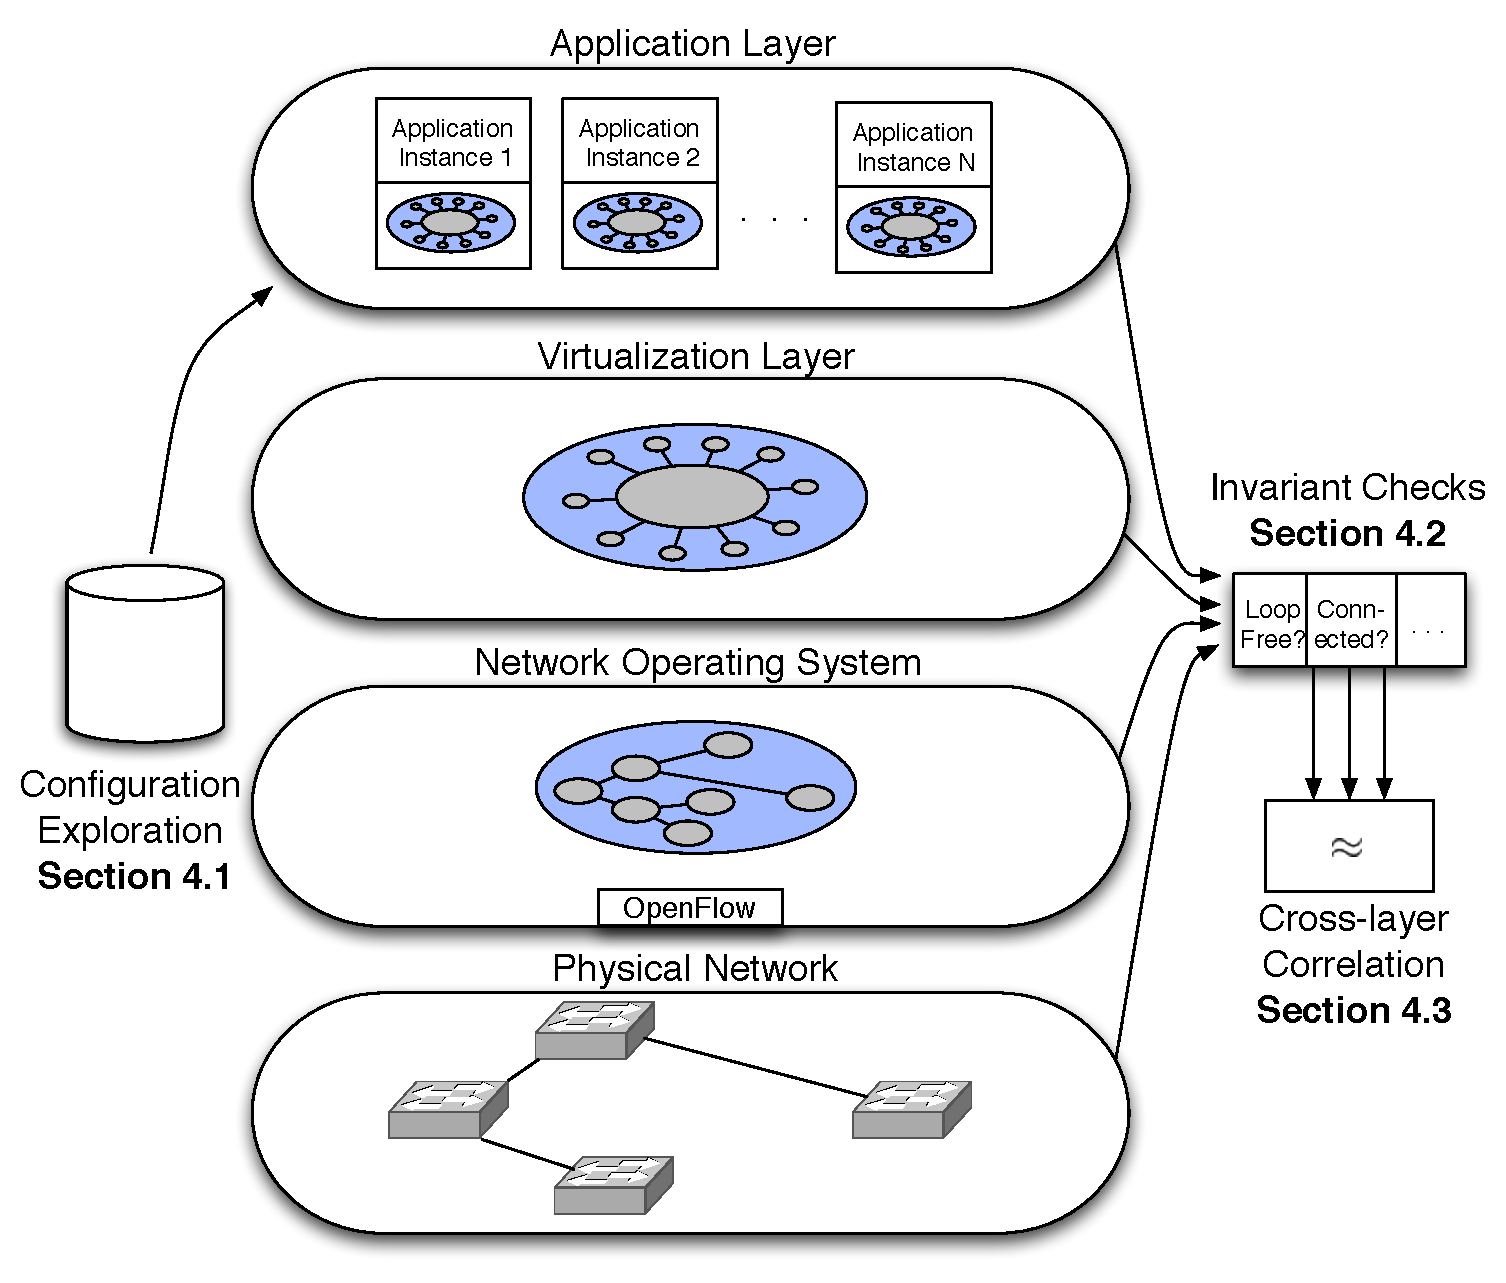
\includegraphics[width=3.25in]{../diagrams/architecture/Architecture_simplified.pdf}
    \caption[]{\label{fig:basicarch} Architectural diagram of \projectname{}, integrated with the SDN stack.} 
\end{figure}

\subsection{Configuration Exploration}
\label{sec:configuration_exploration}

The execution of \projectname{} begins with traffic generation designed to explore the configuration
space of a given control application. 

\projectname{} currently simulates the behavior a physical network in a single-threaded process.
In particular, the NOS and hosted control application are given the illusion that
they are interacting with real network devices. The behavior of the
switches is then mimicked by objects in the same process. We found that
simulation was useful for finding and isolating bugs, since system execution
can be easily logged and deterministically replayed. In the future, we plan to
emulate each network device in a separate process to reproduce the concurrent
nature of software-defined networks.

After an initial network topology has been populated, \projectname{}
generates semi-random packets and delivers them to switches at the border of
the network. As in normal execution, the NOS is notified of these packets, a
control decision is made, and a configuration change is potentially pushed 
to the mock switch objects. We found
that semi-random packet generation suffices to effectively explore the
configuration space of the application. In the future, we plan to explore more
principled input generation, such as trace-driven execution, or symbolic
execution. 

The execution of \projectname{} proceeds in logical rounds. In each round 
a set of events including randomly-generated incoming packets,
switch crashes, controller crashes, and packet drops are generated. Before the end of 
each round, the user is given the opportunity to interactively choose the order
in which the events are executed for that round. We found this useful when we
had a particular failure case in mind, and wanted to easily reproduce the
order of events which lead up to the failure.

\eat{
\colin{TODO: not quite built yet, but it would be easy}
}
\eat{
\colin{Say something about order-independence. That's what makes the input
generator more than just a mechanism to explore the (static) configuration space}
}

\subsection{Invariant Checks}
\label{sec:invariant_checks}

The purpose of the configuration exploration module of \projectname{} was to
infer the behavior of the system under a variety of circumstances. The invariant
checking component of \projectname{} serves to verify the correctness of the
observed system behavior during execution.

We leverage Anteater \cite{anteater}, a static checker for network
dataplanes, to detect the generic failure modes described in Section \ref{sec:bug_analysis}.
At the end of each logical round, we give the user the option of invoking
Anteater's invariant checks. A static snapshot of the mock switches' state is
then taken, translated into RIB format, and fed through Anteater. In our
experience, combining Anteater with configuration exploration is significantly
more effective at detecting errors than Anteater alone.

In addition to the four generic failure modes described in Section
\ref{sec:bug_analysis}, Aneater also allows the user to specify
application-specific invariants with a domain-specific language. In the future
we plan to explore the use of this capability.

\subsection{Cross-layer Correlation}
\label{sec:cross_layer_correlation}

Invariant checking alone does not suffice to detect all possible failure
modes. The NOS itself may fail to configure the physical network in a way that
captures the intended behavior of the control-application. The cross-layer correlation
component of \projectname{} serves to capture such failure-modes. 

Cross-layer correlation involves translating
virtualized representation of the network state to a physical flow table
representation for simulated network elements. It then checks whether there is
there is a one-to-one correspondence between the derived network
state and the true network state.

It should be noted that bugs may exist in the correlation component itself,
especially if the mapping between the virtual and physical network is quite
complex. Nonetheless, we argue that performing this
translation {\it outside} of the system is far more robust than verifying code within the
virtualization layer itself.

\eat{
Consistency checks are a subclass of correspondence checks. If you're running
multiple controllers, it must be the case that either: i. The partitioning of
responsibilities between the controllers is disjoint, or ii. There is a
correspondence between the controllers' views of the network.
}

\subsection{Eventually Consistent NOM}
\begin{figure}[t]
    \hspace{-10pt}
    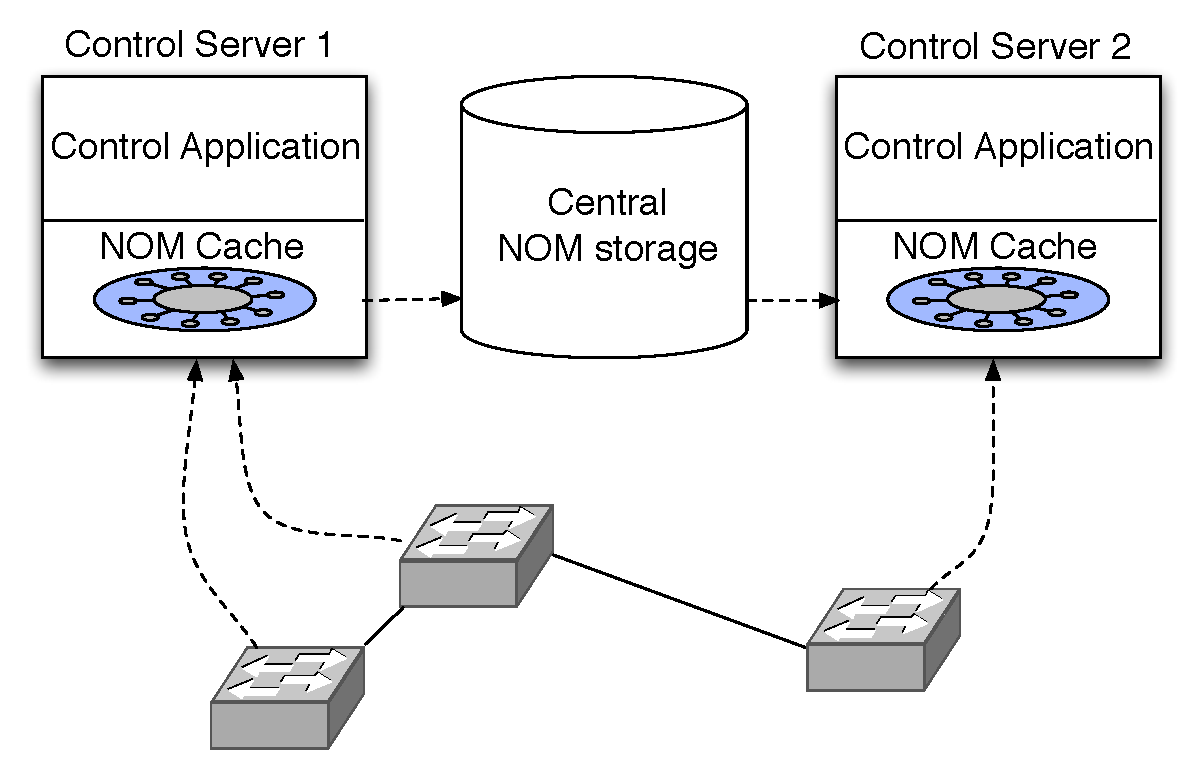
\includegraphics[width=3.25in]{eventually_consistent_nom}
    \caption[]{\label{fig:split_db_nom} Eventually cosnstent NOM from our implementation of a distributed POX controller.} 
\end{figure}


